\documentclass{article}%Formato de plantilla que se utiliza
\usepackage[utf8]{inputenc}%Esto sirve para que nos interprete todos los caracteres en español
\usepackage[spanish]{babel}%Selecciona el lenguaje
\usepackage[margin=2cm, top=2cm, includefoot]{geometry}
\usepackage{graphicx}
\usepackage{subcaption}
\usepackage[table,xcdraw]{xcolor}
\usepackage{tikz,lipsum,lmodern}
\usepackage[most]{tcolorbox}
\usepackage{fancyhdr}
\usepackage{amssymb, amsmath} %Paquetes matemáticos
\usepackage{ragged2e}
\usepackage{multirow}

%declaración de varbiales
\newcommand{\hyperlogo}{img/hyperlogo.png}
\newcommand{\logoUpiita}{img/ulogo.png}
\newcommand{\logoIPN}{img/ilogo.png}
\newcommand{\practica}{Práctica n}%Numero de actividad
%definición de colores
\definecolor{doradoPortada}{HTML}{c7b438}
\definecolor{cherry}{HTML}{6d1741}
\definecolor{blanco}{HTML}{FFFFFF}
\definecolor{morado}{HTML}{c099c6}
%adicionales
\addto\captionsspanish{\renewcommand{\contentsname}{Índice}}
\pagestyle{fancy}
\setlength{\headheight}{58pt}
\setlength{\parindent}{1cm}
\fancyhf{}
%s\rhead{\includegraphics[width=0.155\textwidth]{\logoIPN}}
\lhead{
\includegraphics[width=0.18\textwidth]{\hyperlogo}}
\renewcommand{\headrulewidth}{3pt}
\renewcommand{\headrule}{\hbox to\headwidth {\color{morado}\leaders\hrule height\headrulewidth\hfill}}
%\lfoot{Juan Manuel Mejia Pérez}
\rfoot{\thepage}

\begin{document}%Aquí empieza todo el documento
\begin{titlepage}
\centering

\includegraphics[width=0.8\textwidth]{\hyperlogo}\par\vspace{1cm}
{\huge\bfseries{Hypernova Aerospace}}\par\vspace{0.4cm}
{\scshape{\large ENMICE}}\par\vspace{3cm}
{\bfseries{\huge Reporte de diseño de TonaQube}}\par\vspace{2cm}

%{\scshape{\large Práctica 3 y 4.}}\par\vspace{3cm}
%{\huge \practica}\par\vspace{3cm}
\begin{flushleft}
\begin{tcolorbox}[enhanced jigsaw,breakable,pad at break*=1mm,
  colback=morado,colframe=white!25!black,title=\scshape\large Equipo,
  watermark color=white]
{\scshape\textcolor{blanco}{\normalsize Mejia Pérez Juan Manuel}}\par
{\scshape\textcolor{blanco}{\normalsize }}\par
\end{tcolorbox}\par\vspace{1cm}
\vfill
\end{flushleft}
{\large 18 de septiembre del 2023}
\end{titlepage}
%----------------------------------------------------------------------------------------------------------
\clearpage
\section{Anetecedetes.}
\subsection{Introducción}
\justify
TonaQube es la carga útil que se presentará en ENMICE. Consiste en un satélite
educativo que sigue el factor de forma PocketQube y que su misión es la adquisición
y distribución de señales ambientales para tener conocimiento sobre la calidad del 
aire en la región de lanzamiento y también funcionará como un satélite de observación de
bajo costo.
\subsection{Factor de forma PocketQube}
\justify
El factor de forma PocketQube establece que una unidad debe cumplir con las siguientes 
características:
\begin{itemize}
  \item 5 cm cúbicos
  \item Masa menor igual a 250g
\end{itemize}
\justify
La idea es que 8 unidades de PocketQube quepan dentro de una unidad de CubeSat. La Figura \ref{fig:pq} 
muestra una ilustración de una unidad de PocketQube.
\begin{figure}[!h]
  \centering
  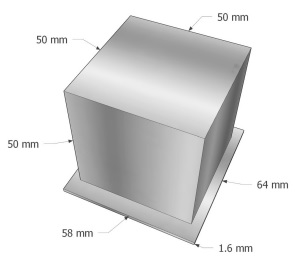
\includegraphics[width=0.5\linewidth]{img/1UPocketQube.jpg}
  \caption{Fotografía de un PocketQube}
  \label{fig:pq}
\end{figure}
\justify
Las ventajas de este tipo de satélite están en el costo, tiempo de desarrollo y la masa. Cuando 
se trata de enviar cosas al espacio, se cobra por Kg de masa que se envía. Por lo que una masa 
baja, reduce el costo de poner el satélite en el espacio para que cumpla su función. El tiempo 
de desarrollo de este tipo de satélites llega a reducirse hasta 1 año de desarrollo en comparación 
de los satélites convencionales que son gigantescas masas tecnológicas que llevan años de desarrollo 
y millones de dólares americanos. 
\subsection{Calidad del aire y sus varbiales}
\justify
La calidad del aire se refiere a la condición o pureza del aire en un lugar determinado. Para
determinar la calidad del aire, se deben medir varias variables ambientales clave como:
\begin{itemize}
  \item Concentración de contaminantes. Implica medir la cantidad de contaminantes presentes en el aire, 
  como partículas en suspensión, óxidos de nitrógeno, dióxido de azufre, monóxido de carbono, ozono y 
  compuestos orgánicos volátiles.
  \item Partículas en suspensión. La medición de partículas finas y gruesas es esencial, ya que pueden tener efectos 
  perjudiciales en la salud huma y el medio ambiente.
  \item Temperatura y humedad. Estas variables pueden influir en la dispersión de contaminantes en el aire 
  y en la formación de ciertos contaminantes atmosféricos, como el ozono.
  \item Velocidad y dirección del viento. Estos factores son importantes para comprender cómo se mueven 
  los contaminantes en la atmósfera y cómo pueden afectar diferentes áreas.
  \item Radiación solar. La cantidad de radiación solar puede influir en la formación de ozono y en 
  la calidad del aire en general.
  \item Contaminantes biológicos. También es importante medir la presencia de contaminantes biológicos, como polen
  y esporas de moho, que pueden afectar la calidad del aire y desencadenar alergias.
\end{itemize}
\justify
La calidad del aire se evalúa en función de los niveles de contaminantes presentes y se compara con estándares y pautas 
pautas establecidos por las autoridades ambientales para determinar si el aire es seguro para la salud humana y el medio 
ambiente. La mejora de la calidad del aire es fundamental para proteger la seguridad pública y el entorno natural.\par
\justify
En México, la Comisión Federal para la Protección contra Riesgos Sanitarios, establece las pautas mostradas en la 
tabla \ref{table:NOMAQ}.

\begin{table}[!h] 
  \begin{center}
    \begin{tabular}{| c | c | c | c | c | c |}
      \hline
      CONTAMINANTE & EVALUACIÓN & EXPOSICIÓN & FRECUENCIA & LÍMITE & NOM \\ \hline
      Partículas PM10 & Promedio 24 hrs & Aguda & No se permite & 75 $\dfrac{\mu g}{m^3}$ & 025-SSA1-2014\\ \hline
      Partículas PM10 & Promedio 24 hrs & Crónica & Promedio anual & 40 $\dfrac{\mu g}{m^3}$ & 025-SSA1-2014\\ \hline
      Partículas PM2.5 & Promedio 24 hrs & Aguda & No se permite & 45 $\dfrac{\mu g}{m^3}$ & 025-SSA1-2014\\ \hline
      Partículas PM2.5 & Promedio 24 hrs & Crónica & Promedio anual & 12 $\dfrac{\mu g}{m^3}$ & 025-SSA1-2014\\ \hline
      Ozonono ($O_3$) & Dato horario & Aguda & No se permite & 0.095 ppm & 020-SSA1-2014 \\ \hline
      Ozonono ($O_3$) & Promedio de 8 hrs & Aguda & No se permite & 0.070 ppm & 020-SSA1-2014 \\ \hline
      ($SO_2$) & Promedio de 8 hrs & Aguda & 1 vez al año & 0.200 ppm & 022-SSA1-2010 \\ \hline
      ($SO_2$) & Promedio de 8 hrs & Aguda & No se permite & 0.110 ppm & 022-SSA1-2010 \\ \hline
      ($SO_2$) & Dato horario & Crónica & -- & 0.025 ppm & 022-SSA1-2010 \\ \hline
      ($NO_2$) & Dato horario & Aguda & 1 vez al año & 0.210 ppm & 023-SSA1-1993 \\ \hline
      ($CO$) & Promedio de 8 hrs & Aguda & 1 vez al año & 11 ppm & 021-SSA1-1993 \\ \hline
      ($Pb$) & Promedio de 3 meses & Crónica & No se permite & 1.5 $\dfrac{\mu g}{m^3}$ & 026-SSA1-1993 \\ \hline
      
    \end{tabular}
    \caption{Normas mexicanas sobre la calidad del aire}
    \label{table:NOMAQ}
  \end{center}
\end{table}

\end{document}